\section{Feature implementation}
Given the start and end time of a call we must compute the cost depending on how many seconds are overlapping the peak period and on how many seconds are overlapping the off-peak period. To apply this change, we initially created two methods in the Call class that calculate and return the peak seconds and the off-peak seconds of the specific call. These methods are called in the BillingSystem class where we get the final cost of the call by multiplying the peak seconds returned with the specific tariff peak rate and the peak seconds with the off-peak seconds.

Having these in mind we initially converted the system milliseconds for the start and end call events into DateTime objects (using the DateTime constructor) that provides us with essential methods that are used to implement the feature.

More specifically the durationPeakSeconds() and  durationOffPeakSeconds() methods were created in the Call class. In the first method we essentially calculate the seconds of the call duration and check how many of them overlap the peak period from 7:00 to 19:00. Taking in to consideration the fact that a call duration can last more than 24 hours, more actions should be taken. One of them was to find out if and how many days existed in call duration. Next, we created a loop that iterates through the days where we create an Interval object for the peak periods for each day. Using those Interval types we compute the seconds that overlap the peak period for every day in the call. An example of the peak seconds calculation is shown below:

\begin{lstlisting}
for (int i=0;i<=daysBetween;i++){
	Interval peakHours=new Interval(peakStart.plusDays(i),peakEnd.plusDays(i));
	Interval overlapWithPeak = callInterval.overlap(peakHours);
	if (overlapWithPeak != null)
		peakSeconds+=overlapWithPeak.toDuration().getStandardSeconds();
}
\end{lstlisting}

For finding the off-peak seconds all we have to do is calculate the duration of the call in seconds and from them just subtract the peak seconds that were computed in the previous method. In the end, all that is left are the seconds overlapping the off-peak period.

Before we started analysing possible solutions for this problem we illustrated the problem by drawing a call timeline across many days, marking the intervals for OffPeak and Peak hours and then “executing” random scenarios on it. You can see an example in the following diagram

\begin{center}
	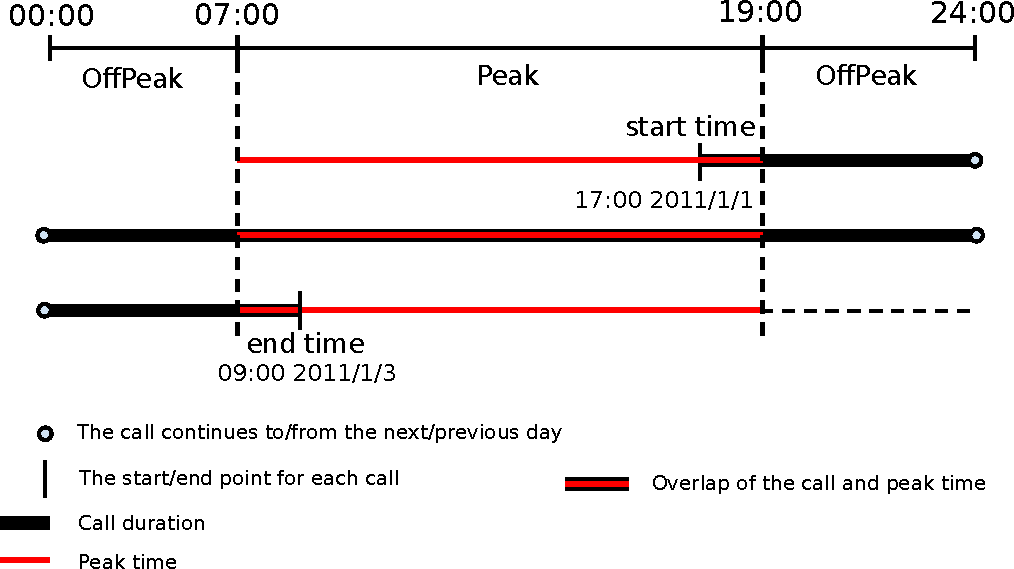
\includegraphics[scale=0.75]{images/timeline.pdf}
\end{center}

In the above diagram we simulate the case when the call starts at 17:00 in a specific day, and ends 2 days after at 05:00 and therefore lasting more than 24 hours. In this particular case we calculate the whole duration between the 2 dates in seconds which are exactly 129600 seconds (36 hours total). We then create 3 peak periods for each day and using the overlap method we calculate all the seconds from the call duration that overlap the peak periods. After computing the peak seconds we also compute the off-peak seconds by subtracting the peak seconds from the whole call duration.
